\chapter{Testování}
Testování systému je jedna z~nejdůležitějších částí navrhování jakýchkoliv systémů.
Správným otestováním by se měla odladit většina potenciálních chyb.



%SECTION
\section{Domácí testování}
Průběžné testování částí webu probíhalo již při~vývoji a~kontrolovalo správné fungování nových funkcí.

Později bylo nutné nachystat rozsáhlejší testy a~připravit jim testovací databázi s~fiktivními daty.
Tímto způsobem jsem například kontroloval správnost běhu funkce pro výpočet času zastavení stroje.

% \begin{figure}[htbp]
%     \centering
%     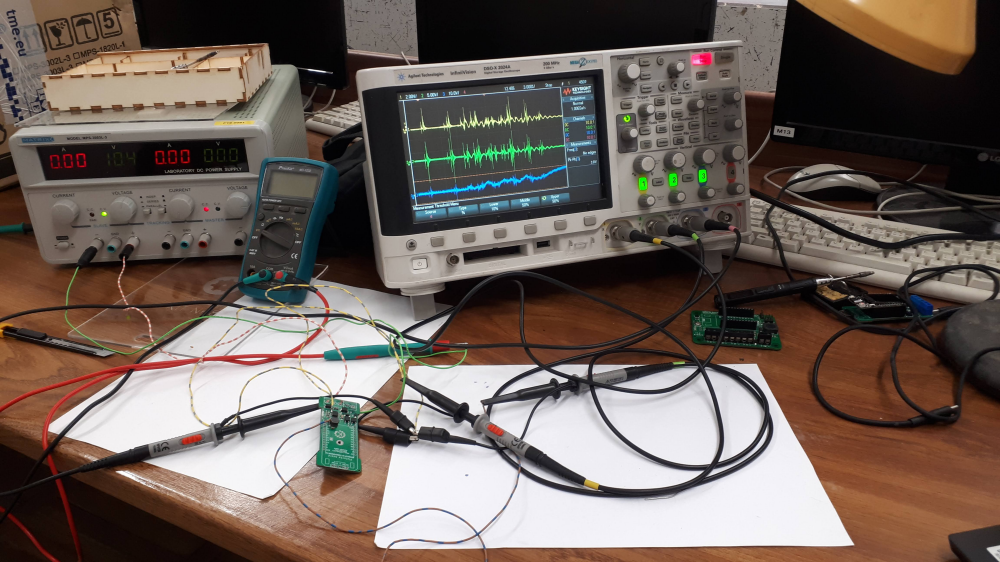
\includegraphics[width=\textwidth]{img/Testovani.png}
%     \caption{Testování senzoru}
%     \label{fig:SenzorNaStroji}
% \end{figure}

\begin{figure}[htbp]
    \centering
    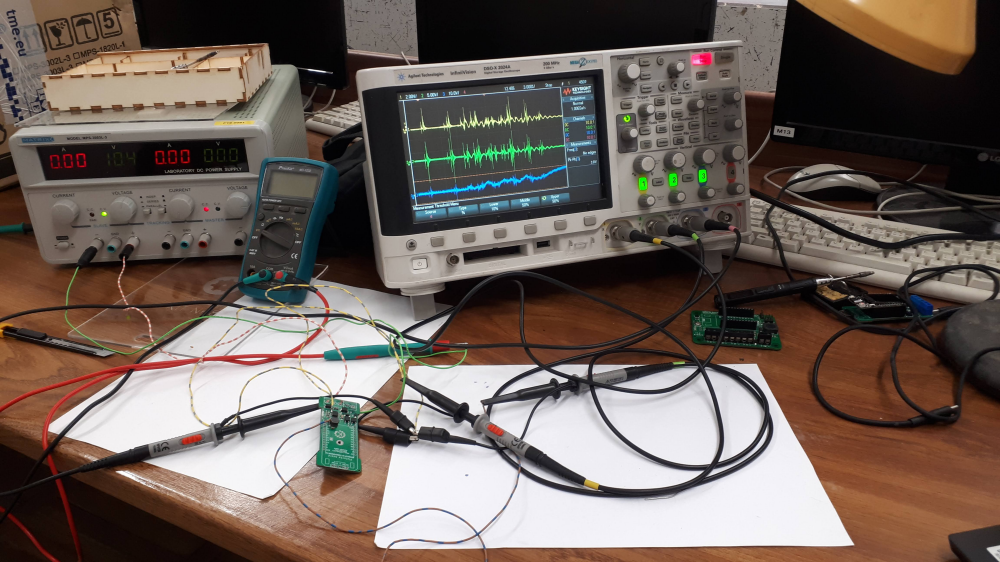
\includegraphics[width=\textwidth]{img/testovani.png}
    \caption{Testování senzoru}
    \label{fig:SenzorNaStroji}
\end{figure}

%SECTION
\section{Testování ve firmě}
V~květnu roku 2020, kdy byly odladěny chyby, jsem systém Pletačka IoT nasadil na dva pletací stroje.
Nově nasbíraná data byla již reálná a~dalo se na nich postavit nové testování.
Senzory jsem nechal několik dní sbírat údaje o~upletených ponožkách a~následně jsem nad nimi spustil generování uživatelsky čitelných dat.

Nasazení dalších senzorů proběhlo koncem září, kdy byly osazeny další dva stroje. 
Byly v provozu čtyři senzory a probíhal vývoj nových.
V půlce prosince jsem připravil dalších šest senzorů a~zahájil dlouhodobé testování bez zásahu do vygenerovaných dat. Naměřené údaje pravidelně stahuji a kontroluji jejich správnost.


